\chapter{Análise Teórica}

A fundamentação analítica desta prática baseia-se na modelagem matemática em alta fidelidade de circuitos ativos de segunda ordem. Ambas as configurações estudadas partem da topologia de Múltipla Realimentação (\textit{Multiple Feedback} — MFB) na configuração inversora. Para viabilizar a resolução analítica das equações diferenciais e a caracterização nos domínios do tempo e da frequência, utilizou-se o ambiente de computação simbólica Maxima \cite{maxima}.

\section{O Amplificador Operacional Ideal}

O amplificador operacional (ampop) é um componente eletrônico de alta complexidade interna, composto por múltiplos estágios de amplificação acoplados em corrente contínua. Para os propósitos da análise linear de circuitos elétricos, adota-se o modelo simplificado do ampop ideal, o qual fornece uma aproximação matemática precisa do comportamento macroscópico do componente em malha fechada.

O ampop ideal consiste essencialmente em um amplificador diferencial cujo comportamento é governado por duas propriedades fundamentais:

\begin{itemize}
	\item \textbf{Resistência de Entrada Infinita ($R_{in} \to \infty$):} Os terminais de entrada comportam-se como um voltímetro ideal. Consequentemente, as correntes de polarização que entram ou saem dos terminais inversor ($v^-$) e não-inversor ($v^+$) são rigorosamente nulas ($i^- = i^+ = 0$).
	\item \textbf{Ganho de Tensão em Malha Aberta Infinito ($A \to \infty$):} A tensão de saída é dada por $V_o = A(V^+ - V^-)$. Para que a tensão de saída permaneça finita e estável sob realimentação negativa, a diferença de potencial entre as entradas deve tender a zero ($\Delta V = V^+ - V^- \to 0$). Esse fenômeno estabelece o conceito de curto-circuito virtual (ou terra virtual quando um dos terminais está aterrado).
\end{itemize}

A Figura \ref{fig:modelo_ampop} ilustra a representação simbólica do ampop ideal e o seu respectivo modelo de circuito equivalente.

\begin{figure}[htbp]
	\centering
	% Substitua pelo nome do arquivo correspondente ao modelo se houver, ou utilize este espaço para o diagrama do ampop
	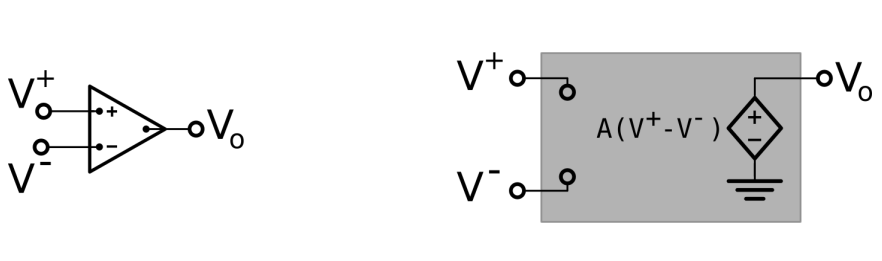
\includegraphics[width=0.6\textwidth]{FIGURAS/modelo_ampop.png}
	\caption{Representação gráfica e modelo de circuito equivalente de um amplificador operacional ideal.}
	\label{fig:modelo_ampop}
\end{figure}

\section{Modelagem Geral da Topologia MFB}

A topologia MFB, apresentada na Figura \ref{fig:esquematico_circuito}, é amplamente utilizada no projeto de filtros ativos por permitir a síntese de polos complexos conjugados utilizando apenas um único elemento ativo. O circuito comporta-se nativamente como um filtro passa-baixa de segunda ordem.

\begin{figure}[htbp]
	\centering
	
\includegraphics[width=0.7\textwidth]{FIGURAS/esquematico_circuito.png}
	\caption{Esquemático elétrico geral do filtro passa-baixa de segunda ordem com Múltipla Realimentação (MFB).}
	\label{fig:esquematico_circuito}
\end{figure}

Considerando o terminal não-inversor conectado diretamente à referência ($V^+ = 0\text{ V}$), o princípio do curto-circuito virtual impõe que o nó inversor atue como um terra virtual ($V^- = 0\text{ V}$). Aplicando a Lei de Kirchhoff das Correntes (LKC) no domínio da frequência complexa $s$ para o nó inversor, obtém-se:

\begin{equation}
	\frac{0 - V_a(s)}{R_3} + (0 - V_o(s))sC_2 = 0 \implies V_a(s) = -V_o(s) \cdot sR_3C_2
	\label{eq:lkc_inversor}
\end{equation}

Analogamente, aplicando a LKC para o nó central de intersecção $V_a(s)$, tem-se:

\begin{equation}
	\frac{V_a(s) - V_i(s)}{R_1} + \frac{V_a(s) - V_o(s)}{R_2} + \frac{V_a(s) - 0}{R_3} + V_a(s)sC_1 = 0
	\label{eq:lkc_no_a}
\end{equation}

Substituindo a relação obtida em \ref{eq:lkc_inversor} na equação nodal \ref{eq:lkc_no_a} e isolando a razão entre a saída e a entrada, determina-se a função de transferência analítica geral do sistema \cite{nilsson}:

\begin{equation}
	H(s) = \frac{V_o(s)}{V_i(s)} = \frac{- \frac{1}{R_1 R_3 C_1 C_2}}{s^2 + s \frac{1}{C_1} \left( \frac{1}{R_1} + \frac{1}{R_2} + \frac{1}{R_3} \right) + \frac{1}{R_2 R_3 C_1 C_2}}
	\label{eq:hs_analitica}
\end{equation}

A partir da estrutura polinomial do denominador, mapeia-se o comportamento padrão de um sistema de segunda ordem através da frequência natural não-amortecida ($\omega_n$) e do fator de amortecimento ($\zeta$), expressos por:

\begin{equation}
	\omega_n = \frac{1}{\sqrt{R_2 R_3 C_1 C_2}}
\end{equation}

\begin{equation}
	\zeta = \frac{\sqrt{R_2 R_3 C_1 C_2}}{2 \cdot C_1} \left( \frac{1}{R_1} + \frac{1}{R_2} + \frac{1}{R_3} \right)
\end{equation}

O ganho estático em corrente contínua (ganho DC, obtido quando $s = 0$) simplifica-se para a relação puramente resistiva $A_v = -R_2/R_1$ \cite{nilsson}.

\section{Primeiro Circuito: Análise do Regime Superamortecido}

O primeiro circuito particular utiliza os seguintes valores nominais de projeto:
\begin{center}
	$R_1 = 47\text{ k}\Omega \quad R_2 = 470\text{ k}\Omega \quad R_3 = 470\text{ k}\Omega \quad C_1 = 100\text{ nF} \quad C_2 = 10\text{ nF}$
\end{center}

Substituindo estes valores na equação geral \ref{eq:hs_analitica} por meio do comando \texttt{at()} do Maxima, encontra-se a seguinte função de transferência numérica:

\begin{equation}
	H_1(s) = \frac{-45269,35}{s^2 + 255,32s + 4526,94}
\end{equation}

As raízes do polinômio característico do denominador determinam os polos do sistema:
\begin{equation}
	s_1 \approx -19,17\text{ rad/s} \quad \text{e} \quad s_2 \approx -236,15\text{ rad/s}
\end{equation}

Dado que ambos os polos são estritamente reais, negativos e distintos, o sistema opera sob o regime \textbf{superamortecido} ($\zeta > 1$). O ganho DC em baixas frequências é de $-10\text{ V/V}$ ($20\text{ dB}$). Devido ao distanciamento entre as raízes, o polo próximo à origem ($s_1$) atua como polo dominante, definindo a frequência de corte de $-3\text{ dB}$ em aproximadamente $3,05\text{ Hz}$ ($19,17\text{ rad/s}$). 

Frente a um estímulo em degrau de $0,8\text{ V}$, a resposta temporal calculada via Transformada Inversa de Laplace apresenta um perfil puramente amortecido e sem oscilações, convergindo para o valor final estável de $-8,0\text{ V}$:

\begin{equation}
	v_{o1}(t) = -8 + 8,706e^{-19,17t} - 0,706e^{-236,15t}
\end{equation}

\section{Segundo Circuito: Análise do Regime Subamortecido}

Para a segunda configuração, os valores de $R_1$ e $R_3$ são permutados entre si, alterando a dinâmica de atenuação e armazenamento de energia:
\begin{center}
	$R_1 = 470\text{ k}\Omega \quad R_2 = 470\text{ k}\Omega \quad R_3 = 47\text{ k}\Omega \quad C_1 = 100\text{ nF} \quad C_2 = 10\text{ nF}$
\end{center}

A substituição destes parâmetros gera a função de transferência numérica:

\begin{equation}
	H_2(s) = \frac{-100000000}{2209s^2 + 564000s + 10000000}
\end{equation}

A resolução do denominador pelo Maxima resulta em um par de polos complexos conjugados:
\begin{equation}
	s_{1,2} \approx -127,66 \pm j171,94\text{ rad/s}
	\label{eq:polos_complexos}
\end{equation}

A presença de componentes imaginárias caracteriza o regime de operação como \textbf{subamortecido} ($0 < \zeta < 1$). Nesta condição, o ganho estático DC cai para a unidade inversora ($-1\text{ V/V}$ ou $0\text{ dB}$). Em contrapartida, o baixo fator de amortecimento induz o surgimento de um pico de ressonância no diagrama de magnitude de Bode. A frequência angular onde ocorre o pico de magnitude máxima ($\omega_{max}$) é calculada analiticamente por:

\begin{equation}
	\omega_{max} = \omega_n \sqrt{1 - 2\zeta^2} \approx 112,58\text{ rad/s} \quad (\approx 17,9\text{ Hz})
\end{equation}

Quando submetido a uma excitação em degrau com amplitude de $5\text{ V}$, o comportamento transitório manifesta uma resposta subamortecida clássica. O sinal de saída ultrapassa temporariamente o valor de regime permanente (apresentando sobressinal ou \textit{overshoot}) e oscila de forma senoidal amortecida antes de convergir para o valor final de $-5\text{ V}$:

\begin{equation}
	v_{o2}(t) = -5 + 5e^{-127,66t} \left[ \cos(171,94t) + 0,742\sin(171,94t) \right]
\end{equation}

\section{Síntese dos Parâmetros Teóricos Calculados}

Para consolidar a análise matemática realizada e estabelecer uma linha de base clara para as etapas subsequentes de medição e pós-processamento, os principais parâmetros obtidos analiticamente para ambos os circuitos foram sintetizados. A Tabela \ref{tab:resumo_teorico} apresenta de forma comparativa as métricas fundamentais do regime permanente em frequência e do regime transitório no tempo.

\begin{table}[htbp]
	\centering
	\caption{Resumo dos parâmetros teóricos calculados via computação simbólica.}
	\label{tab:resumo_teorico}
	\begin{tabular}{lcc}
		\hline
		\textbf{Parâmetro Teórico} & \textbf{Primeiro Circuito} & \textbf{Segundo Circuito} \\ \hline
		Configuração de Amortecimento & Superamortecido & Subamortecido \\ 
		Polos do Sistema ($s$) & $-19,17$ e $-236,15 \text{ rad/s}$ & $-127,66 \pm j171,94 \text{ rad/s}$ \\ 
		Ganho Estático DC ($A_v$) & $-10 \text{ V/V } (20 \text{ dB})$ & $-1 \text{ V/V } (0 \text{ dB})$ \\ 
		Frequência de Corte $-3\text{ dB}$ ($f_1$) & $3,05 \text{ Hz}$ & — \\ 
		Frequência de Pico Máximo ($f_{max}$) & — & $17,9 \text{ Hz}$ \\ 
		Amplitude de Entrada Senoidal ($V_i$) & $0,8 \text{ V}$ & $5,0 \text{ V}$ \\ 
		Amplitude de Saída Máxima Esperada & $8,0 \text{ V}$ & $5,0 \text{ V}$ \\ \hline
		\textbf{Resposta ao Degrau} & \textbf{Degrau de } $0,8\text{ V}$ & \textbf{Degrau de } $5,0\text{ V}$ \\ \hline
		Valor de Convergência Final ($t \to \infty$) & $-8,0 \text{ V}$ & $-5,0 \text{ V}$ \\ 
		Tempo de 10\% do Valor Final & $9,8 \text{ ms}$ & $1,2 \text{ ms}$ \\ 
		Tempo de 90\% do Valor Final & $124,5 \text{ ms}$ & $10,6 \text{ ms}$ \\ 
		Tempo de Acomodação ($\pm 10\%$) & — & $18,0 \text{ ms}$ \\ \hline
	\end{tabular}
\end{table}

Esses índices nominais serão utilizados como referência absoluta durante as atividades práticas em laboratório, permitindo quantificar os desvios percentuais causados pelas tolerâncias intrínsecas dos componentes comerciais utilizados na montagem.